%%%%%%%%%%%%%%%%%%%%%%%%%%%%%%%%%%%%%%%%%
% Beamer Presentation
% LaTeX Template
% Version 1.0 (10/11/12)
%
% This template has been downloaded from:
% http://www.LaTeXTemplates.com
%
% License:
% CC BY-NC-SA 3.0 (http://creativecommons.org/licenses/by-nc-sa/3.0/)
%
%%%%%%%%%%%%%%%%%%%%%%%%%%%%%%%%%%%%%%%%%

%----------------------------------------------------------------------------------------
%	PACKAGES AND THEMES
%----------------------------------------------------------------------------------------

\documentclass{beamer}

\mode<presentation> {

% The Beamer class comes with a number of default slide themes
% which change the colors and layouts of slides. Below this is a list
% of all the themes, uncomment each in turn to see what they look like.

%\usetheme{default}
%%\usetheme{AnnArbor}
%\usetheme{Antibes}
%\usetheme{Bergen}
%\usetheme{Berkeley}
%\usetheme{Berlin}
%\usetheme{Boadilla}
%\usetheme{CambridgeUS}
%\usetheme{Copenhagen}
%\usetheme{Darmstadt}
%\usetheme{Dresden}
%\usetheme{Frankfurt}
%\usetheme{Goettingen}
%\usetheme{Hannover}
%\usetheme{Ilmenau}
%\usetheme{JuanLesPins}
%\usetheme{Luebeck}
\usetheme{Madrid}
%\usetheme{Malmoe}
%\usetheme{Marburg}
%\usetheme{Montpellier}
%\usetheme{PaloAlto}
%\usetheme{Pittsburgh}
%\usetheme{Rochester}
%\usetheme{Singapore}
%\usetheme{Szeged}
%\usetheme{Warsaw}

% As well as themes, the Beamer class has a number of color themes
% for any slide theme. Uncomment each of these in turn to see how it
% changes the colors of your current slide theme.

%\usecolortheme{albatross}
\usecolortheme{beaver}
%\usecolortheme{beetle}
%\usecolortheme{crane}
%\usecolortheme{dolphin}
%\usecolortheme{dove}
%\usecolortheme{fly}
%\usecolortheme{lily}
%\usecolortheme{orchid}
%\usecolortheme{rose}
%\usecolortheme{seagull}
%\usecolortheme{seahorse}
%\usecolortheme{whale}
%\usecolortheme{wolverine}

%\setbeamertemplate{footline} % To remove the footer line in all slides uncomment this line
%\setbeamertemplate{footline}[page number] % To replace the footer line in all slides with a simple slide count uncomment this line

%\setbeamertemplate{navigation symbols}{} % To remove the navigation symbols from the bottom of all slides uncomment this line
}

\usepackage{graphicx} % Allows including images
\usepackage{booktabs}
\usepackage{movie15} % Allows the use of \toprule, \midrule and \bottomrule in tables


%----------------------------------------------------------------------------------------
%	TITLE PAGE
%----------------------------------------------------------------------------------------
\setbeamertemplate{navigation symbols}{} %turn off navigation symbols
\title[General Fusion]{Energy of Tomorrow: General Fusion} % The short title appears at the bottom of every slide, the full title is only on the title page

\author{ Branden Messmer, Ian Rankin, Jerin Roberts} % Your name

\institute[TRU] % Your institution as it will appear on the bottom of every slide, may be shorthand to save space
{


}
\date{\today} % Date, can be changed to a custom date

\begin{document}

\begin{frame}
\centering

\titlepage % Print the title page as the first slide
 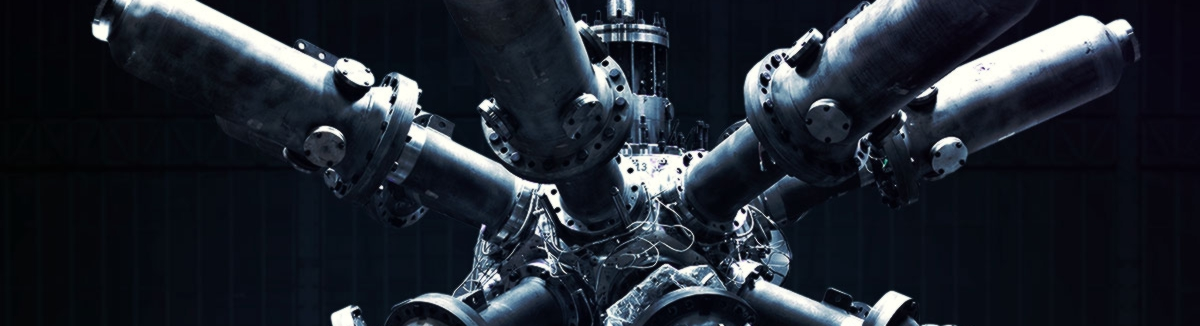
\includegraphics[width=\linewidth]{gf}
\end{frame}

\begin{frame}
\frametitle{Overview} % Table of contents slide, comment this block out to remove it
\tableofcontents % Throughout your presentation, if you choose to use \section{} and \subsection{} commands, these will automatically be printed on this slide as an overview of your presentation
\end{frame}

%----------------------------------------------------------------------------------------
%	PRESENTATION SLIDES
%----------------------------------------------------------------------------------------

%------------------------------------------------
\section{Introduction} % Sections can be created in order to organize your presentation into discrete blocks, all sections and subsections are automatically printed in the table of contents as an overview of the talk
%------------------------------------------------

 % A subsection can be created just before a set of slides with a common theme to further break down your presentation into chunks
\begin{frame}
\frametitle{The Current Situation}
\begin{itemize}
\item U.S. Department of Energy predicts a 50\% increase in global energy consumption by 2035
\item Fossil fuels currently generate the majority of the world’s power
\item What if there was an alternative?
\newline
\center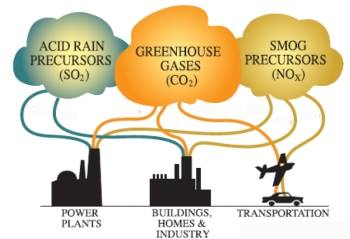
\includegraphics[height=4cm]{fus7}
\end{itemize}
\end{frame}

%------------------------------------------------


\section{What is Fusion?}
\begin{frame}
\frametitle{What is Fusion?}
\begin{itemize}
\item A constituent of the Atom is the nucleus
\item Composed of nucleons$:$ protons, neutrons
\item Nuclei can be split or fused, resulting in heat energy
\item This energy arises from the interaction of two forces
\item Nucleons exert a binding force amongst themselves at very close distances and protons exert a columbic repulsion
\item Energy source of stellar bodies
\newline
\center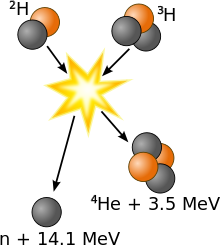
\includegraphics[height=3cm]{fus5}\space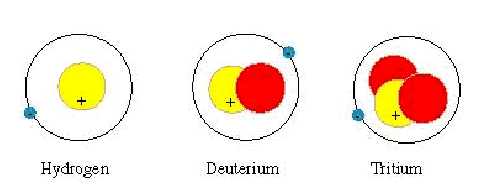
\includegraphics[height=3cm]{fus4.png}

\end{itemize}
\end{frame}

\section{Why is Fusion Important?}
\begin{frame}
\frametitle{Why is Fusion Important?}
\begin{itemize}
\item Energy Consumption/ Population Growth
\item Abundant/Accessible Fuel
\item Low Pollution
\newline
\center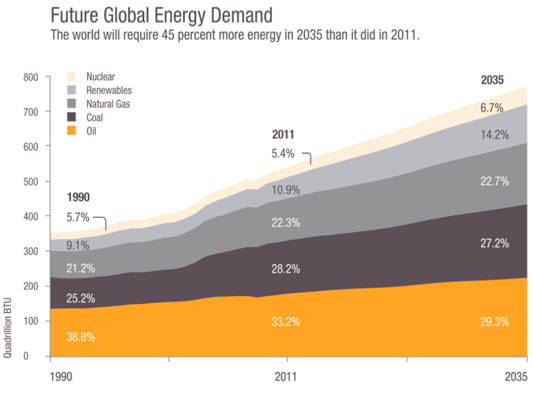
\includegraphics[height=5cm]{fus6}
\end{itemize}
\end{frame}
%------------------------------------------------
\section{Why Don't We Have it?}
\begin{frame}
\frametitle{Why Don't We Have it?}
\begin{itemize}
\item Fusion only occurs naturally in stars
\item Technology to generate and withstand extreme conditions is complex
\item $Energy_{in} < Energy_{out}$
\item Multiple reactor designs
\newline
\center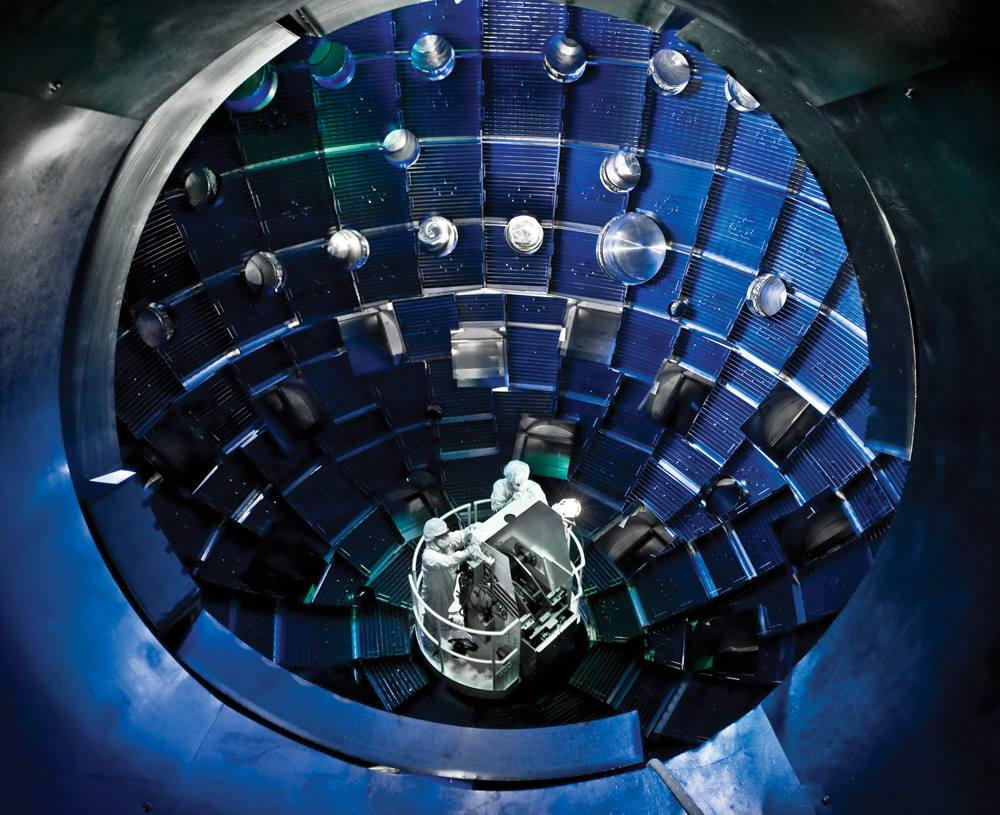
\includegraphics[height=4cm]{fus8}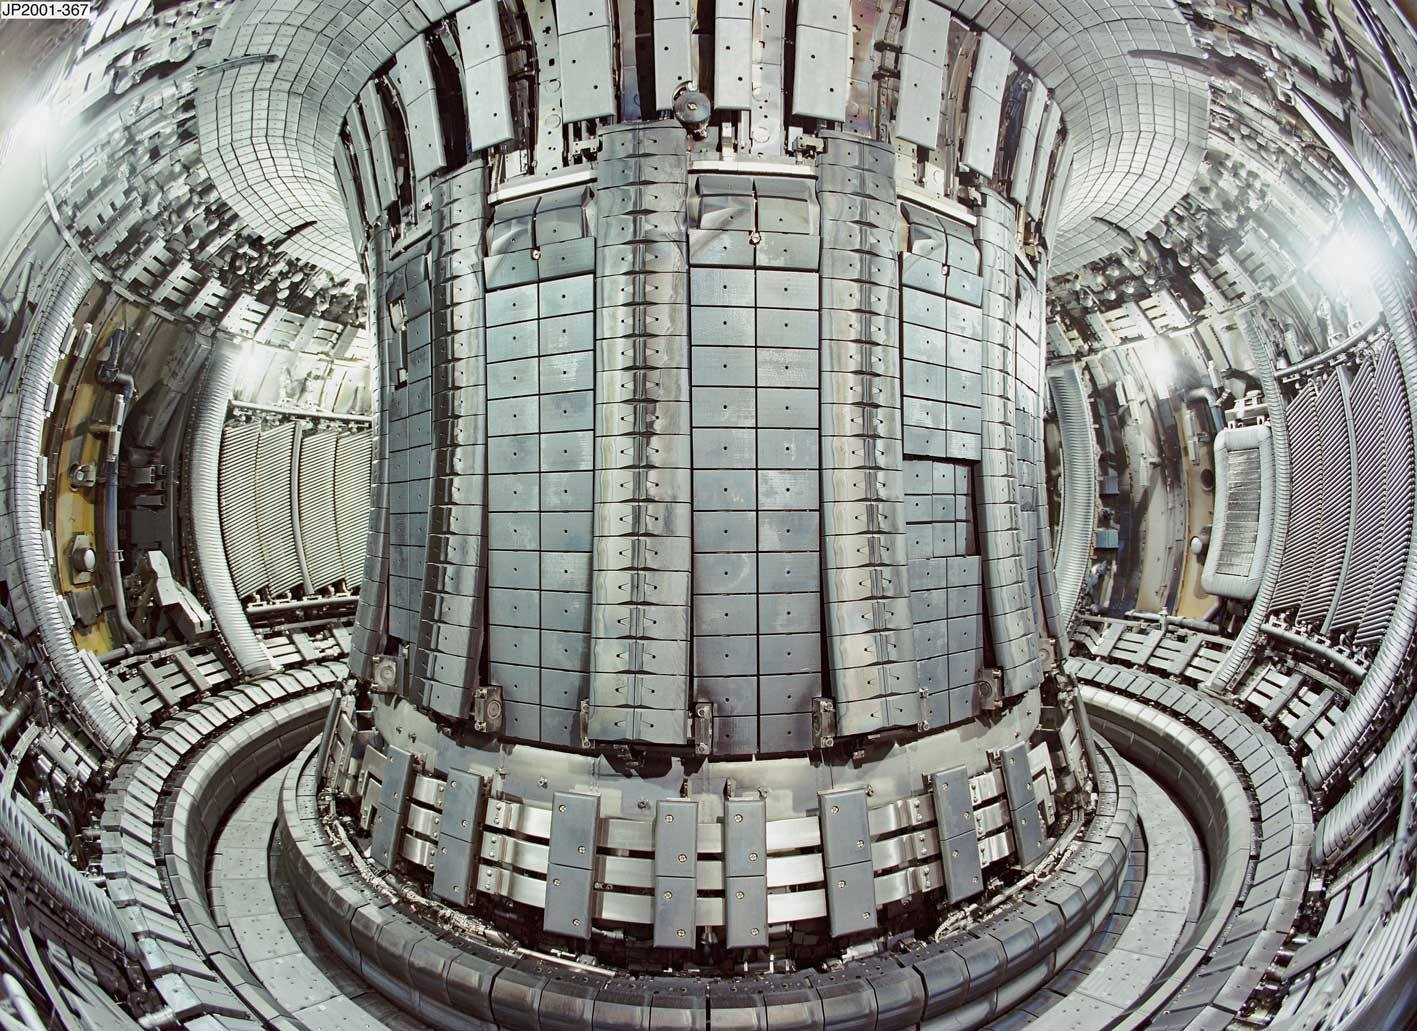
\includegraphics[height=4cm]{fus9}
\end{itemize}
\end{frame}

\section{Progress Towards Fusion}
\begin{frame}
\frametitle{Progress Towards Fusion}
\begin{itemize}
\item Multiple reactors internationally
\item General Fusion
\item Magnetized target fusion
\item Reactor design
\begin{itemize}
\item Pistons slam into liquid lead alloy filled shell
\item Pressure waves catalyze fusion of Deuterium and Tritium
\item Liquid lead absorbs and exchanges heat
\item Breeds one of the fuel ingredients
\item Smaller/cheaper than other reactors
\end{itemize}
\center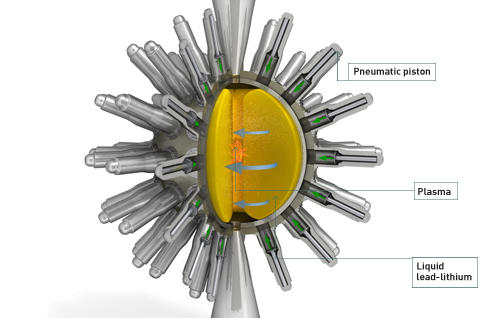
\includegraphics[height=3cm]{fus1}
\end{itemize}
\end{frame}

\section{Advantages of General Fusions Reactor}
\begin{frame}
\frametitle{Advantages of General Fusions Reactor}
\begin{itemize}
\item Small Cheap reactor
\item Direct Energy extraction from Liquid Lead
\item Tritium Breeding from Neutron Bombardment
\item Scale Reactor Construction in Progress
\center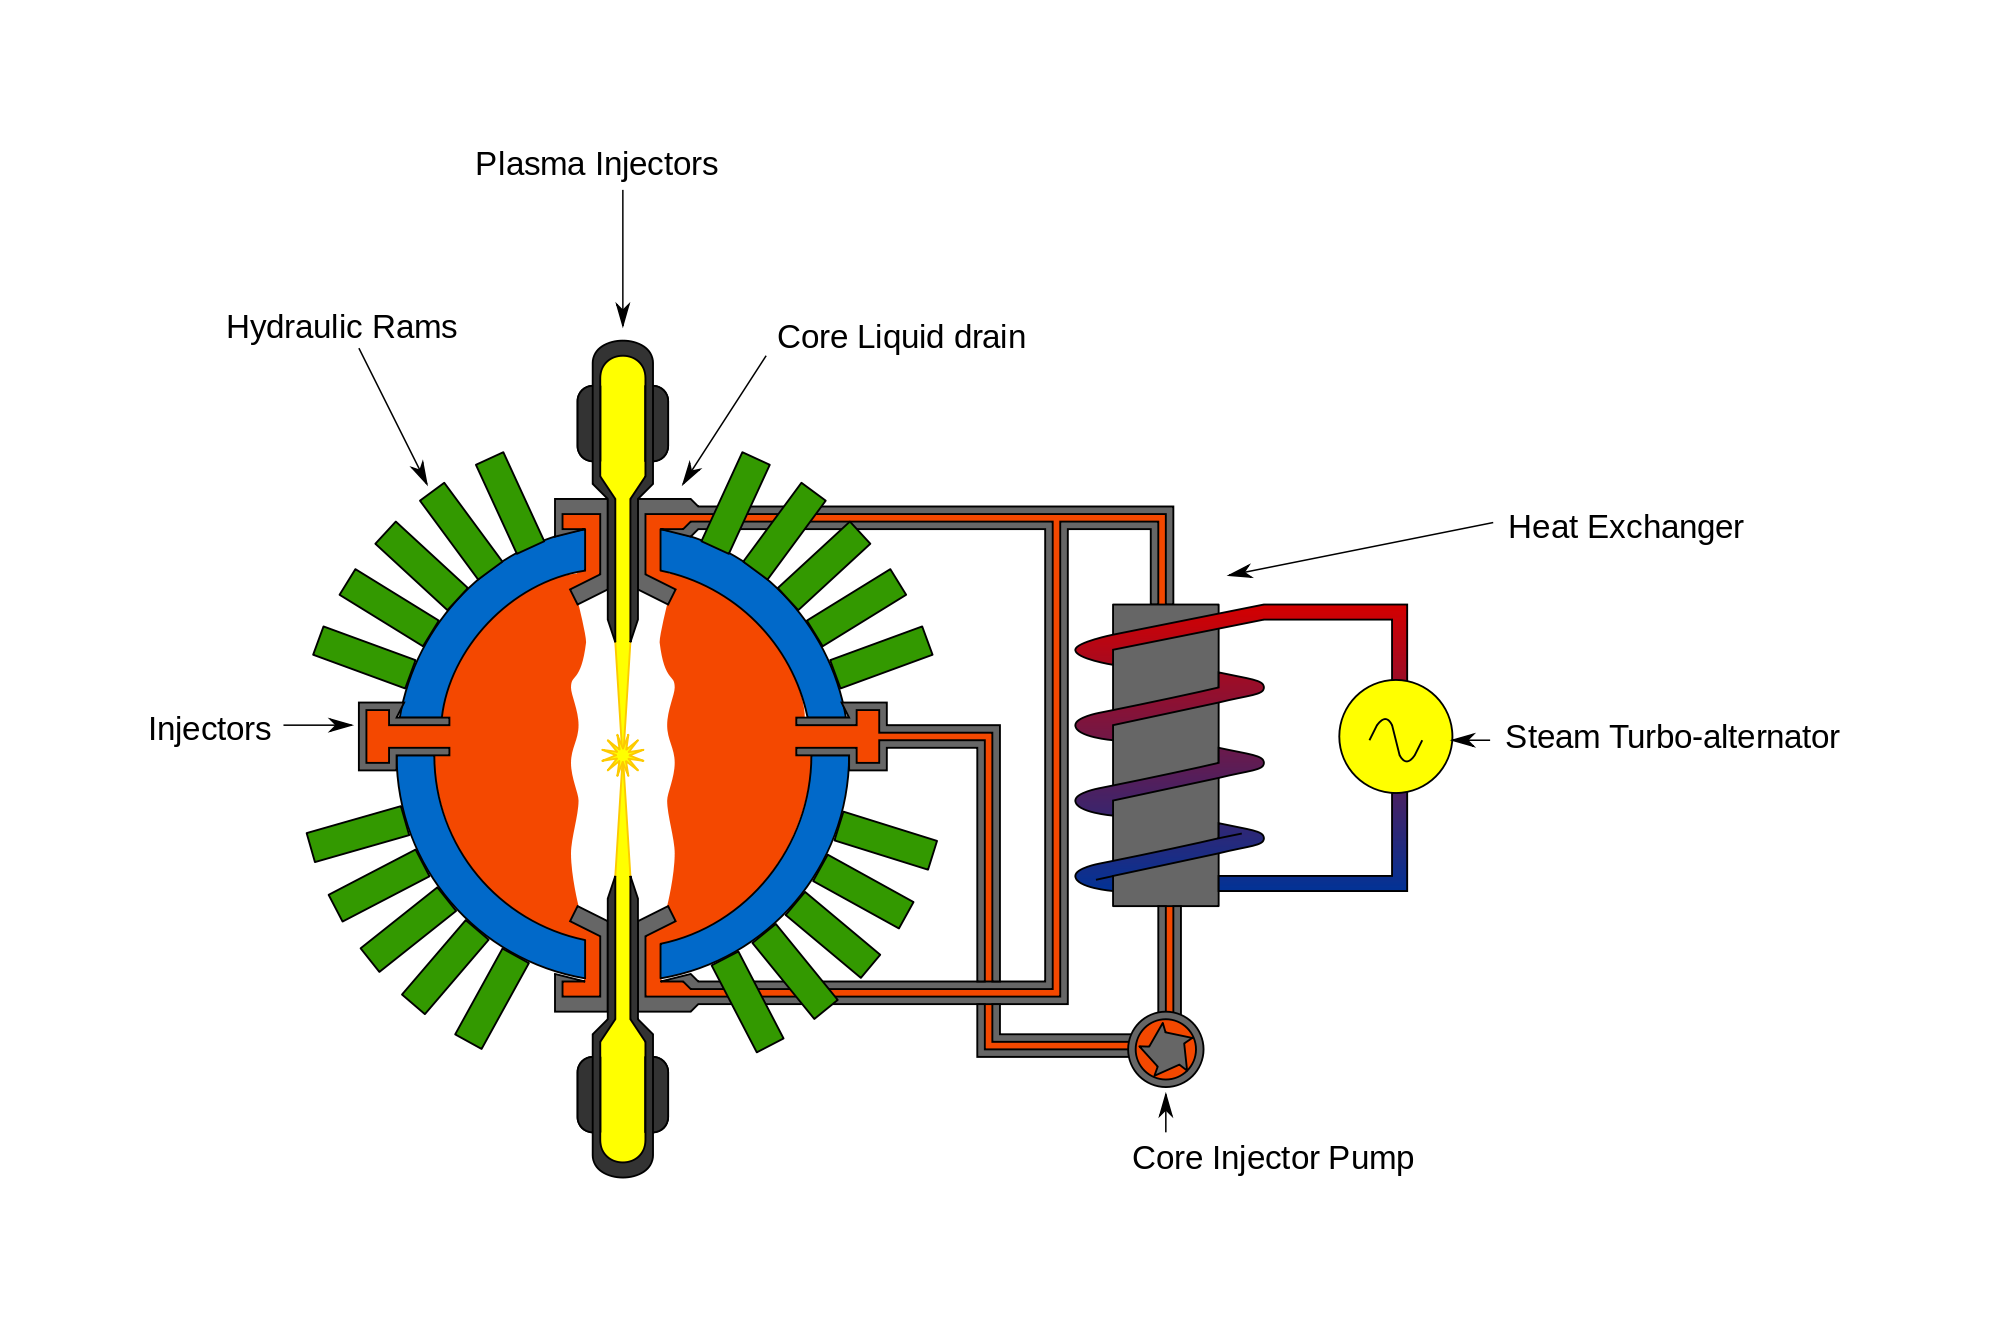
\includegraphics[height=6cm]{fus2}
\end{itemize}
\end{frame}

\section{Final Thoughts}
\begin{frame}
\frametitle{Final Thoughts}
\begin{itemize}
\item Fusion Provides Answer to Growing Energy Demand
\item Abundant and Clean Fuel Source
\item Only Technical Issues hindering Progress
\item General Fusion Provides answer for Cheap Efficient Reactor 
\newline
\center
\includegraphics[height=3cm]{fus3}
\end{itemize}
\end{frame}

\begin{frame}
\frametitle{References}
\footnotesize{
\begin{thebibliography}{99} % Beamer does not support BibTeX so references must be inserted manually as below
\bibitem[Smith, 2013]{p1} Laberge, Michel (2009)
\newblock "An Acoustically Driven Magnetized Target Fusion Reactor."  AIP Conference Proceedings
\newblock 7/26/2009, Vol. 1154 Issue 1, p282-288. 7p. 4

\bibitem[Sawan, 2014]{p1} Sawan M.E. (2006)
\newblock  "Physics and technology conditions for attaining tritium self-sufficiency for the DT fuel cycle." Fusion Engineering and Design
\newblock [accessed 2014 Feb 2] 81:1131-1144

\bibitem[Smith, 2013]{p1} Flavio Dobran (2012)
\newblock "Fusion Energy Conversion In Magnetically Confined Plasma Reactors."  Progress In Nuclear Energy
\newblock 8/2012, Vol. 60, p89-116



\end{thebibliography}
}
\end{frame}

%------------------------------------------------

\begin{frame}
\Huge{\centerline{Thank-you}}
\end{frame}

%----------------------------------------------------------------------------------------



\end{document} 